From the given information, 
 $\triangle PQR$ is a right angled triangle. Let $QR=p$ and $\theta$=30$\degree$.
Then the vertices of the triangle are
\begin{align}
\vec{P} &= \myvec{0\\0} \\
\vec{Q} &= \myvec{0 \\ p \cos \theta } \\
	&= \myvec{0 \\ 4.07} \\
\vec{R} &= \myvec{p \sin \theta \\ 0}\\
	&= \myvec{2.35 \\ 0}
\end{align}
The triangle is plotted in Fig. \ref{constr/tri/27/2/fig}
%
\begin{figure}[ht]
  \centering
    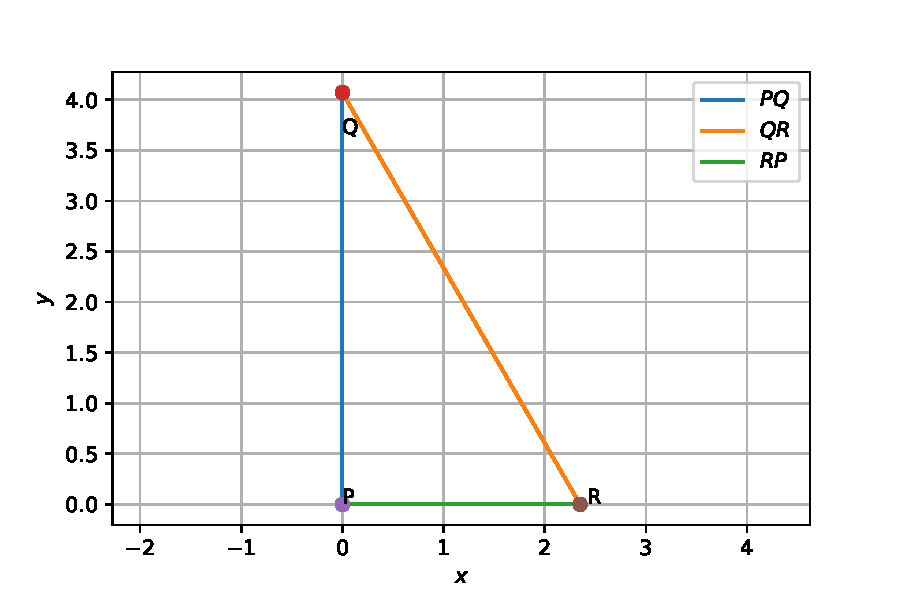
\includegraphics[width= \columnwidth]{solutions/triangle/27/2/triangle1.pdf}
    \caption{$\triangle PQR$ constructed using python}
    \label{constr/tri/27/2/fig}
\end{figure}
